%
% PROJECT: <ETD> Electronic Thesis and Dissertation Initiative
%   TITLE: LaTeX report template for ETDs in LaTeX
%  AUTHOR: Neill Kipp, nkipp@vt.edu
%     URL: http://etd.vt.edu/latex/
% SAVE AS: etd.tex
% REVISED: September 6, 1997 [GMc 8/30/10]
% 

% Instructions: Remove the data from this document and replace it with your own,
% keeping the style and formatting information intact.  More instructions
% appear on the Web site listed above.

\documentclass[12pt,dvips]{report}

\usepackage{fullpage}
%\usepackage{natbib}
%\usepackage{breakurl}
\usepackage{algorithmic}
\usepackage{alltt}
\usepackage[ruled]{algorithm2e}
\usepackage[cmex10]{amsmath}
\usepackage{url} 
\usepackage{graphicx}
\usepackage{listings}
\usepackage{wrapfig}
\usepackage{multirow}
%\usepackage[plainpages=false, colorlinks=true, urlcolor={cyan}, citecolor={red}, linkcolor={green}]{hyperref}
\usepackage[plainpages=false]{hyperref}
\usepackage{array}
\usepackage{balance}
\usepackage{subfigure}
\usepackage{amssymb}
\usepackage{float}
%\usepackage{caption}
\usepackage{placeins}
\usepackage{harmony}

% % % % % % % % % % % % % % % % % % % % % % % % % % % % % % % % 
\lstset{frame=none, xleftmargin=15pt, stepnumber=1, numbers=left, numbersep=5pt,
numberstyle=\tiny, belowcaptionskip=\bigskipamount,
captionpos=b, escapeinside={*'}{'*}, language=java, tabsize=2, emphstyle={\bf},
commentstyle=\it, stringstyle=\mdseries\ttfamily, showspaces=false,
keywordstyle=\bfseries, morekeywords={in,do,print,Metadata,Where}, columns=flexible,
basicstyle=\footnotesize\ttfamily, showstringspaces=false, morecomment=[l], mathescape=true}



% \newcommand{\solution}{\bigskip\hrule\bigskip}
% \newcommand{\problembreak}{\bigskip\hrule\bigskip}

% \renewcommand{\theenumi}{\bf\Alph{enumi}}

% \newlength{\spread}
% \setlength{\spread}{1.0in}

% \def\bibfont{\footnotesize}

% correct bad hyphenation here
%\hyphenation{op-tical net-works semi-conduc-tor}


%%%%%%%%%%%%%%%%%%%%%%% END of LaTeX definitions %%%%%%%%%%%%%%%%%%%%%%%%%%%%

\setlength{\textwidth}{6.5in}
\setlength{\textheight}{8.5in}
\setlength{\evensidemargin}{0in}
\setlength{\oddsidemargin}{0in}
\setlength{\topmargin}{0in}

\setlength{\parindent}{0pt}
\setlength{\parskip}{0.1in}

% Uncomment for double-spaced document.
% \renewcommand{\baselinestretch}{2}

% \usepackage{epsf}

\begin{document}

\thispagestyle{empty}
\pagenumbering{roman}
\begin{center}

% TITLE
{\Large 
Musiplectics: Computational Assessment of the Complexity of Music Scores
}

\vfill

Ethan G. Holder

\vfill

Dissertation submitted to the Faculty of the \\
Virginia Polytechnic Institute and State University \\
in partial fulfillment of the requirements for the degree of

\vfill

Masters of Science \\
in \\
Computer Science

\vfill

Eli Tilevich, Chair \\
Amy Gillick \\
R. Ben Knapp

\vfill

April 23, 2015 \\
Blacksburg, Virginia

\vfill

Keywords: Music Scores; Music Complexity Assessment; Novel Computing Domains; MusicXML
\\
Copyright 2015, Ethan G. Holder

\end{center}

\pagebreak

\thispagestyle{empty}
\begin{center}

{\large Musiplectics: Computational Assessment of the Complexity of Music Scores}

\vfill

Ethan G. Holder

\vfill

(ABSTRACT)

\vfill

\end{center}

In the Western classical tradition, musicians play music from notated sheet music, called a score. When playing music from a score, a musician translates its visual symbols into sequences of instrument-specific physical motions. Hence, a music score's overall complexity represents a sum of the cognitive and mechanical acuity required for its performance.
For a given instrument, different notes, intervals, articulations, dynamics, key signatures, and tempo represent dissimilar levels of difficulty, which vary depending on the performer's proficiency. Individual musicians embrace this tenet, but may disagree about the degrees of difficulty.

This paper introduces \emph{musiplectics}\footnote{musiplectics = music + plectics, Greek for the study of complexity}, a systematic and objective approach to computational assessment of the complexity of a music score for any instrument. Musiplectics defines computing paradigms for automatically and accurately calculating the complexity of playing a music score on a given instrument. The core concept codifies a two-phase process. First, music experts rank the relative difficulty of individual musical components (e.g., notes, intervals, dynamics, etc.) for different playing proficiencies and instruments. Second, a computing engine automatically applies this ranking to music scores and calculates their respective complexity. As a proof of concept of musiplectics, we present an automated, Web-based application called Musical Complexity Scoring (MCS) for music educators and performers. Musiplectics can engender the creation of practical computing tools for objective and expeditious assessment of a music score's suitability for the abilities of intended performers.

This thesis is based on research submitted for publication at ONWARD'15.

\vfill

% GRANT INFORMATION

That this work received support from a Virginia Tech ICAT SEED grant.

\pagebreak

% Dedication and Acknowledgments are both optional

\chapter*{Dedication}

\thispagestyle{empty}

\begin{center}

\vfill

%This thesis is dedicated to the memories of Robert Brooks Nance, Katherine Gayle Nance, and Durward Alexander Holder. You are deeply loved and sorely missed.  

%\textit{To the memories of Robert Brooks Nance, Katherine Gayle Nance, and Durward Alexander Holder; I sorely miss and deeply love you all.}

\vfill

\end{center}

\pagebreak

\chapter*{Acknowledgments}

\thispagestyle{empty}

This thesis would not have been possible without the generous help of many people. First and foremost, I would like to thank my research advisor, Dr. Eli Tilevich, for taking a chance on me as a student, guiding me through the publication process, and supporting me throughout my studies. I owe a great deal of thanks to Dr. Cliff Shaffer, a dedicated professor and reference, who has encouraged me to get involved in research in only my first semester as an undergraduate. I must also thank the numerous professionals that advocated the research process as both an undergraduate and graduate student, including Mr. Mack McGhee, Mrs. Andrea Bailey, and Mr. Adrian Rodriguez.

I generously thank my fellow researchers, Eeshan Shah and Mohammed Davoodi, without whom much of this research would not have been possible. I must express significant thanks to all of the other various professors and advisors who have worked with me over my years at Virginia Tech. Among all of these, I would be remiss if I did not expressly thank Mrs. Terry Arthur. Your guidance from the very first time I met you, before I even began classes, all the way through until my end as an undergraduate has been outstanding in every way.

Last but not least, I must thank all of my family and friends who pushed me to achieve as much as I have. I especially thank my mother, Laurel Holder, and father, Mark Holder, for instilling a love of learning in me from a very young age and for constantly encouraging me even when I had stumbled along my way. I owe it all to you, and I can never thank you enough.

\pagebreak

\tableofcontents
\pagebreak

\listoffigures
\pagebreak

\listoftables
\pagebreak

\pagenumbering{arabic}
\pagestyle{myheadings}

\chapter{Introduction}
\markright{Ethan G. Holder  \hfill Chapter 1. Introduction \hfill}

Which piano concerto is more difficult: Rachmaninoff’s Second or Third? A newly appointed band director wonders if this new orchestral score is appropriate for a high school band, given that the clarinet and bassoon sections are quite advanced, while the flute and oboe sections are more novice. Music educators working on pedagogical guidelines for K-12 students are trying to decide whether a given piece belongs in the N or N+1 curricular level. A publisher wonders which audience to target when marketing new works, while the publisher's customers face great uncertainty when determining whether unfamiliar music matches their playing ability. Performers, band directors, educators, and publishers encounter these non-trivial questions throughout their professional careers. 


Unfortunately, determining the relative complexity of music is a non-trivial cognitive task. Additionally, methods in the current state of the art depend solely on individual opinions, a process influenced by personal biases and lacking common criteria. In other words, the only way to answer these questions in a viable way is to carefully analyze music scores by hand, a tedious, error-prone, and time-consuming process. The stakeholders at hand would rather spend their precious time on more creative pursuits.

Can computing help decode these persistent and challenging questions? Is it possible to provide such technology in a ubiquitous and user-friendly way, accessible to any interested musician? To answer these questions, this paper presents musiplectics, a new computational paradigm, that systematically evaluates the relative difficulty of music scores, thus benefiting educators and performers. Two insights provide a foundation behind musiplectics. First, certain notes and other musical components, including intervals, dynamics, and articulations, are harder to play than the others. Second, automated computer processing can transform a prohibitively tedious, error-prone, and subjective process into a practical and pragmatic solution if exposed via an intuitive user interface. Hence, musiplectics fuses commonly accepted music tenets and novel computing paradigms, to objectively answer the questions above. 


Musiplectics draws its inspiration from computational thinking \cite{wing2006computational}. The problem of estimating the expected performance efficiency of a given program has been studied in great detail. We have computational approaches that can predict the amount of computational resources that will be required to execute a program. By tallying the costs of individual instructions, one can estimate the overall cost of executing a program on a given platform. Analogously, individual musical components also have agreed upon costs, defined in terms of the difficulty they present to performers. By decomposing a music score into its individual musical components, one can use their unit costs to compute the total complexity of executing a score on a given instrument, as shown in Figure \ref{image:analogy}.

%While this work may seem like it addresses an unorthodox software engineering problem, in fact determining the relative complexity of music has many analogues in software. Consider figure \ref{image:complexities} which shows the different types of complexity associated with playing music. It also shows one typical scenario for generating output from high-level code. In both the cognitive tasks of decoding high-level code and reading music notes, relatively short, expressive statements are transformed into complex actions to be performed. Then both take those actions and perform them to generate some kind of output. 

% \begin{figure}[ht!]
% 	\centering
% 		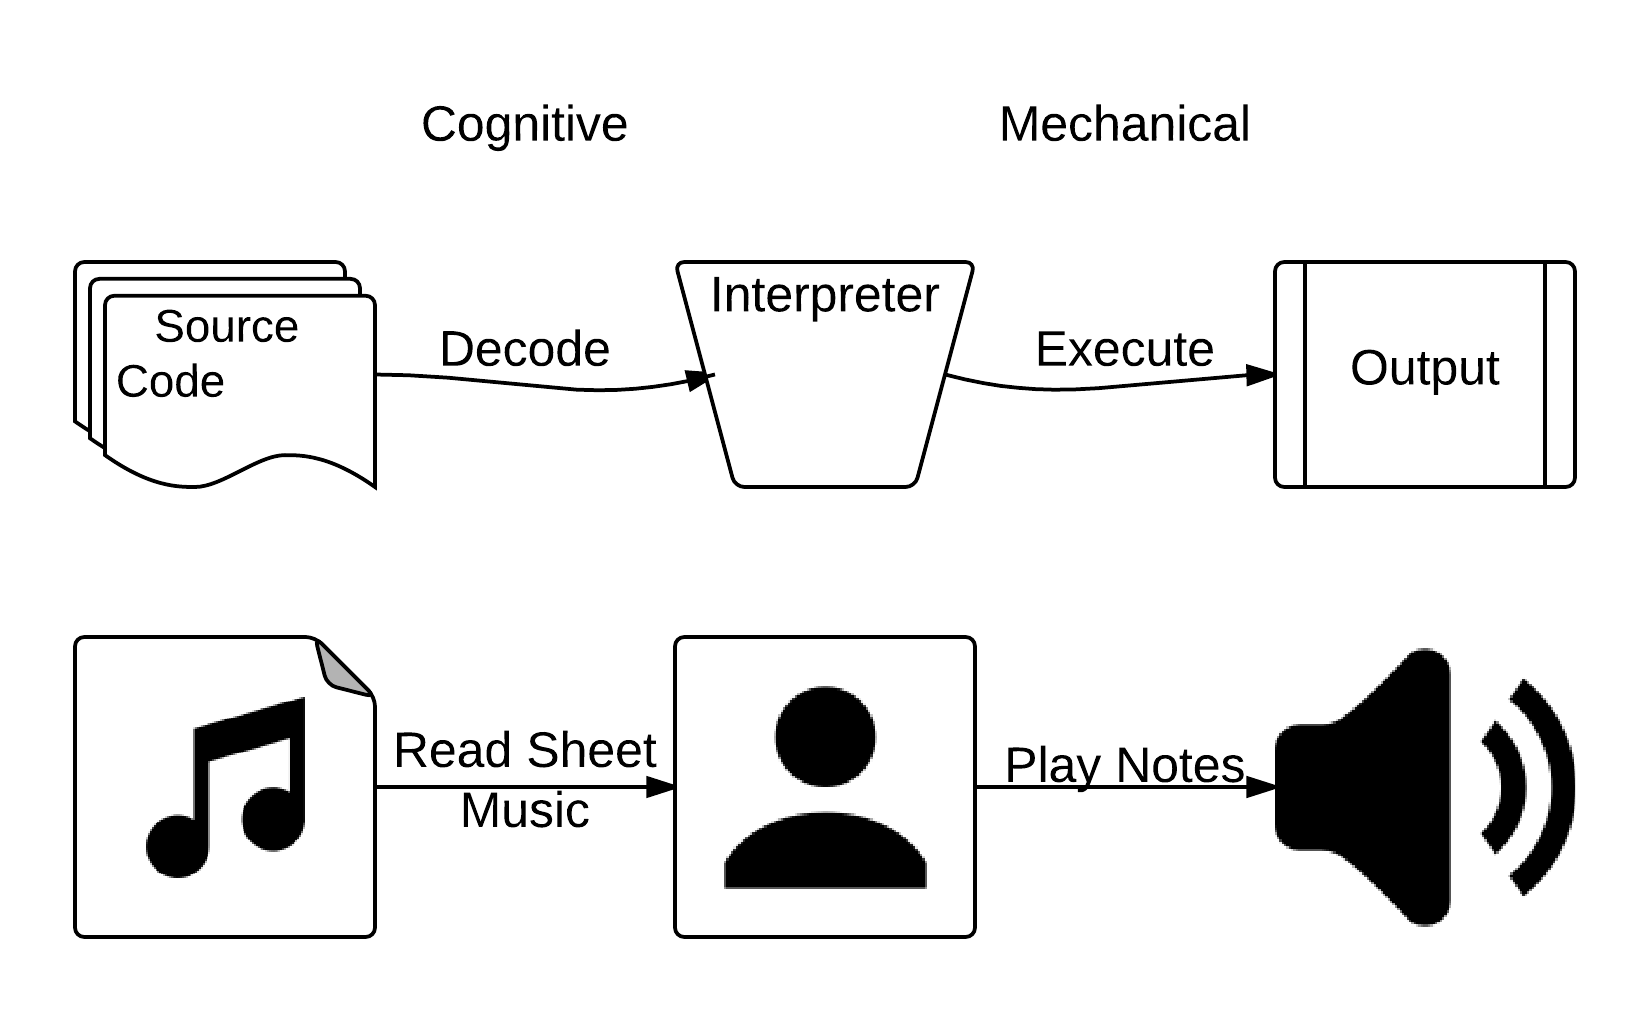
\includegraphics[width=0.47\textwidth]{CognitiveMechanical.png}
% 		\caption{The process of playing music introduces cognitive and mechanical complexities in reading and playing notes, respectively, just like interpreting high-level code into a virtual machine and executing it to produce output.}
% 		\label{image:complexities}
% \end{figure} 

\begin{figure}
	\hfill
		\caption{The process of decomposing code and music to extrapolate a conclusion.}
		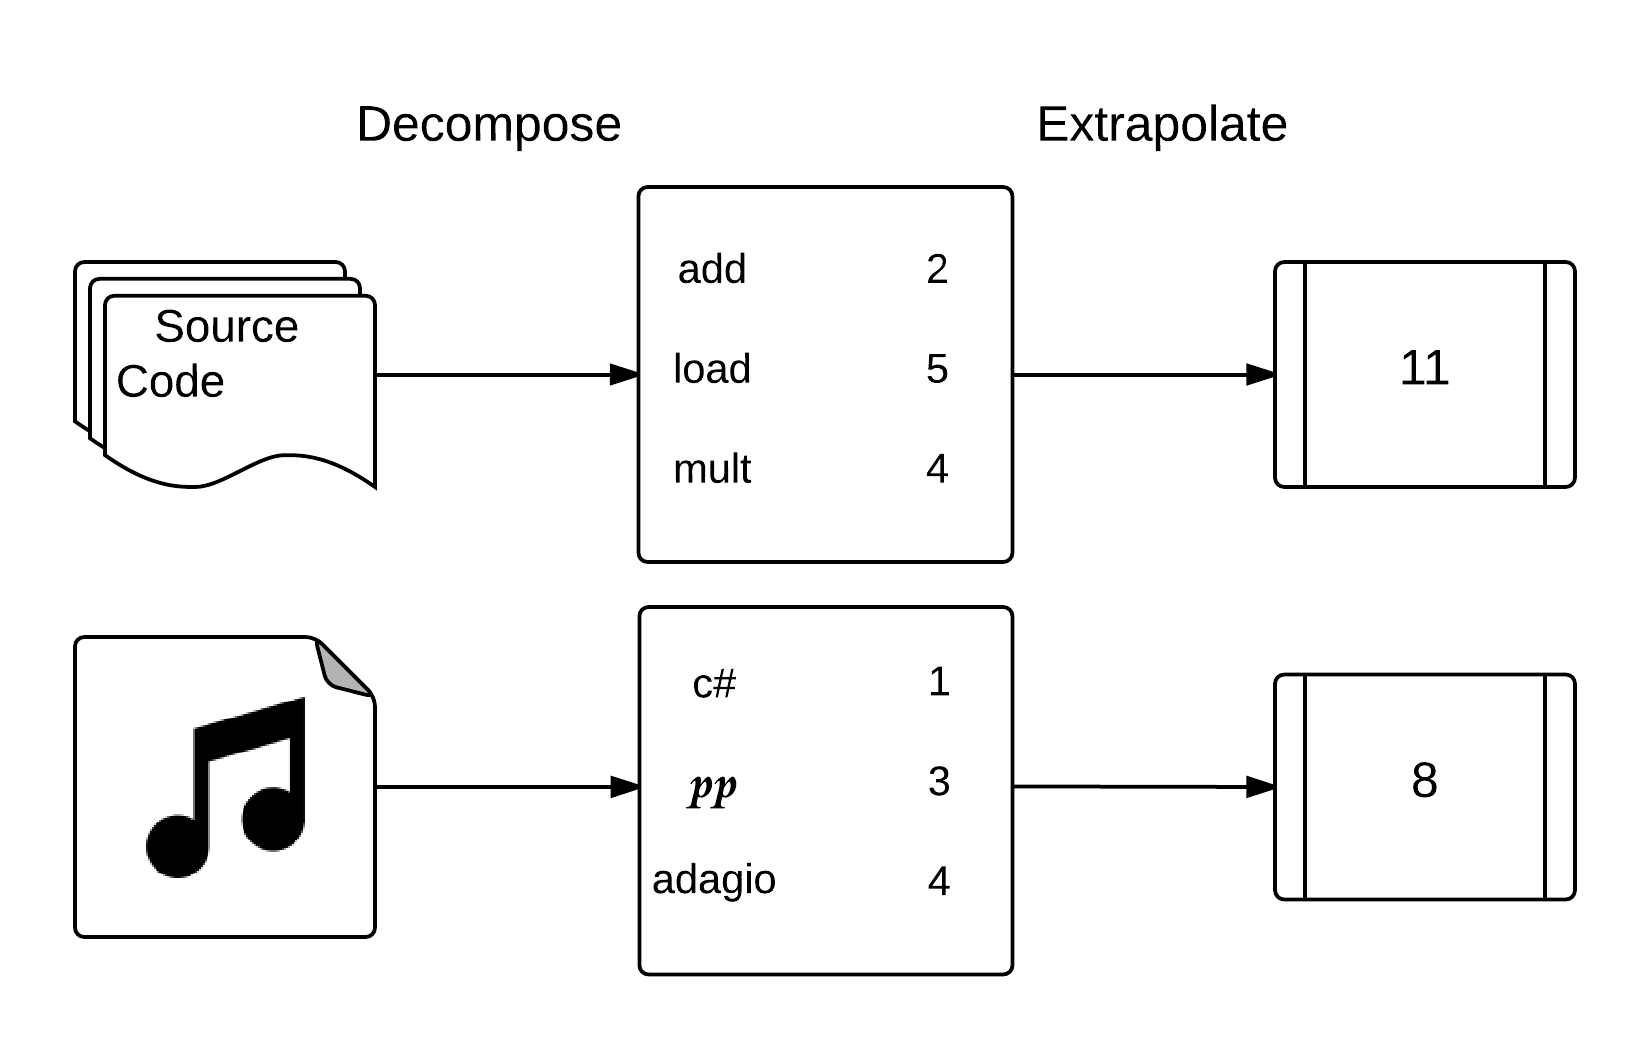
\includegraphics[width=0.8\textwidth,natwidth=1650,natheight=1050]{ComputationalThinkingAnalogy.png}
		\label{image:analogy}
	\hfill
\end{figure} 

Although one can draw various analogies between music and computing, the intricacy of determining the complexity of music scores is most similar to estimating program performance on different computing devices. While the same compiled program can be executed on any computing device of a given architecture, the device's processing power ultimately determines the efficiency of the resulting execution, which can vary widely. The same applies to the complexity experienced by musicians with dissimilar levels of proficiency when performing the same piece on a given instrument. Although all musicians read a piece of sheet music and understand it similarly, the complexity of playing that piece is determined by a performer's proficiency. Musiplectics aspires to blaze a trail toward objectively assessing these complexities by creating a practical computational framework that can capture the subtle nuances of musical complexity.

The solutions presented herein are instrument agnostic. Nevertheless, to realize the concept of musiplectics, our reference implementation of the computational framework targets the B$\flat$ Clarinet. This exclusive focus on clarinet is reflective of our own music performance expertise, rather than of any limitations of the presented concepts.

%%%%%%%%%%%%%%%%%
%
% Include an EPS figure with this command:
%   \epsffile{filename.eps}
%

%%%%%%%%%%%%%%%%
%
% Do tables like this:

 \begin{table}
 \caption{The Graduate School wants captions above the tables.}
\begin{center}
 \begin{tabular}{ccc}
 x & 1 & 2 \\ \hline
 1 & 1 & 2 \\
 2 & 2 & 4 \\ \hline
 \end{tabular}
\end{center}
 \end{table}

%%%%%%%%%%%%%%%%%%%%%%%%%%%%%%%%

% If you are using BibTeX, uncomment the following:

\nocite{*}
\bibliographystyle{abbrvnat}
\thebibliography{HolderThesis2015}
%\bibliography{HolderThesis2015}

% Otherwise, uncomment the following:
% \chapter*{Bibliography}

% \appendix

% In LaTeX, each appendix is a "chapter"
% \chapter{Program Source}


\end{document}